\documentclass[../main.tex]{subfiles}

\begin{document}
\section{Why Mutual \texorpdfstring{\( k \)}{k}-Nearest Neighbours Graphs?}
As stated in \cref{sec:prior work}, the first approach to identify clusters and outliers
in a dataset was by finding the maximal cliques of the Mutual \( k \)-Nearest Neighbours
graph, \MKNN graph for short. Let's describe how it is constructed to better understand
its usefulness. 

One starts with the Nearest Neighbours graph. Given a point cloud, \( C
\), its Nearest Neighbour directed graph is constructed according to the following
prescription: there is an edge from \( p \) to \( q \) if and only if \( d(p,q) = \min_{r
	\in C} d(p,r) \), so \( q \) is the closest point to \( p \), its \emph{nearest
neighbour}. The reason the graph is directed is because the relation of being a nearest
neighbour is not symmetric (think of three points, two of which are close together, while
the third one is far away: the firs two are nearest neighbours of each other, and the
third is a nearest neighbour of one of the first two, but not the other way around). 

This generalises to the \( k \)-Nearest Neighbours graph, in which each point is connected
to its \( k \)-th nearest neighbours, that is, the \( k \)-th closest points to it. The
resulting graph is still directed. We obtain the undirected \emph{Mutual} \( k \)-Nearest
Neighbours graph by connecting two points if and only if there are edges between them
in both directions, i.e. if they are \emph{mutual} \( k \)-nearest neighbours. 

\begin{figure}[htb]
	\centering
	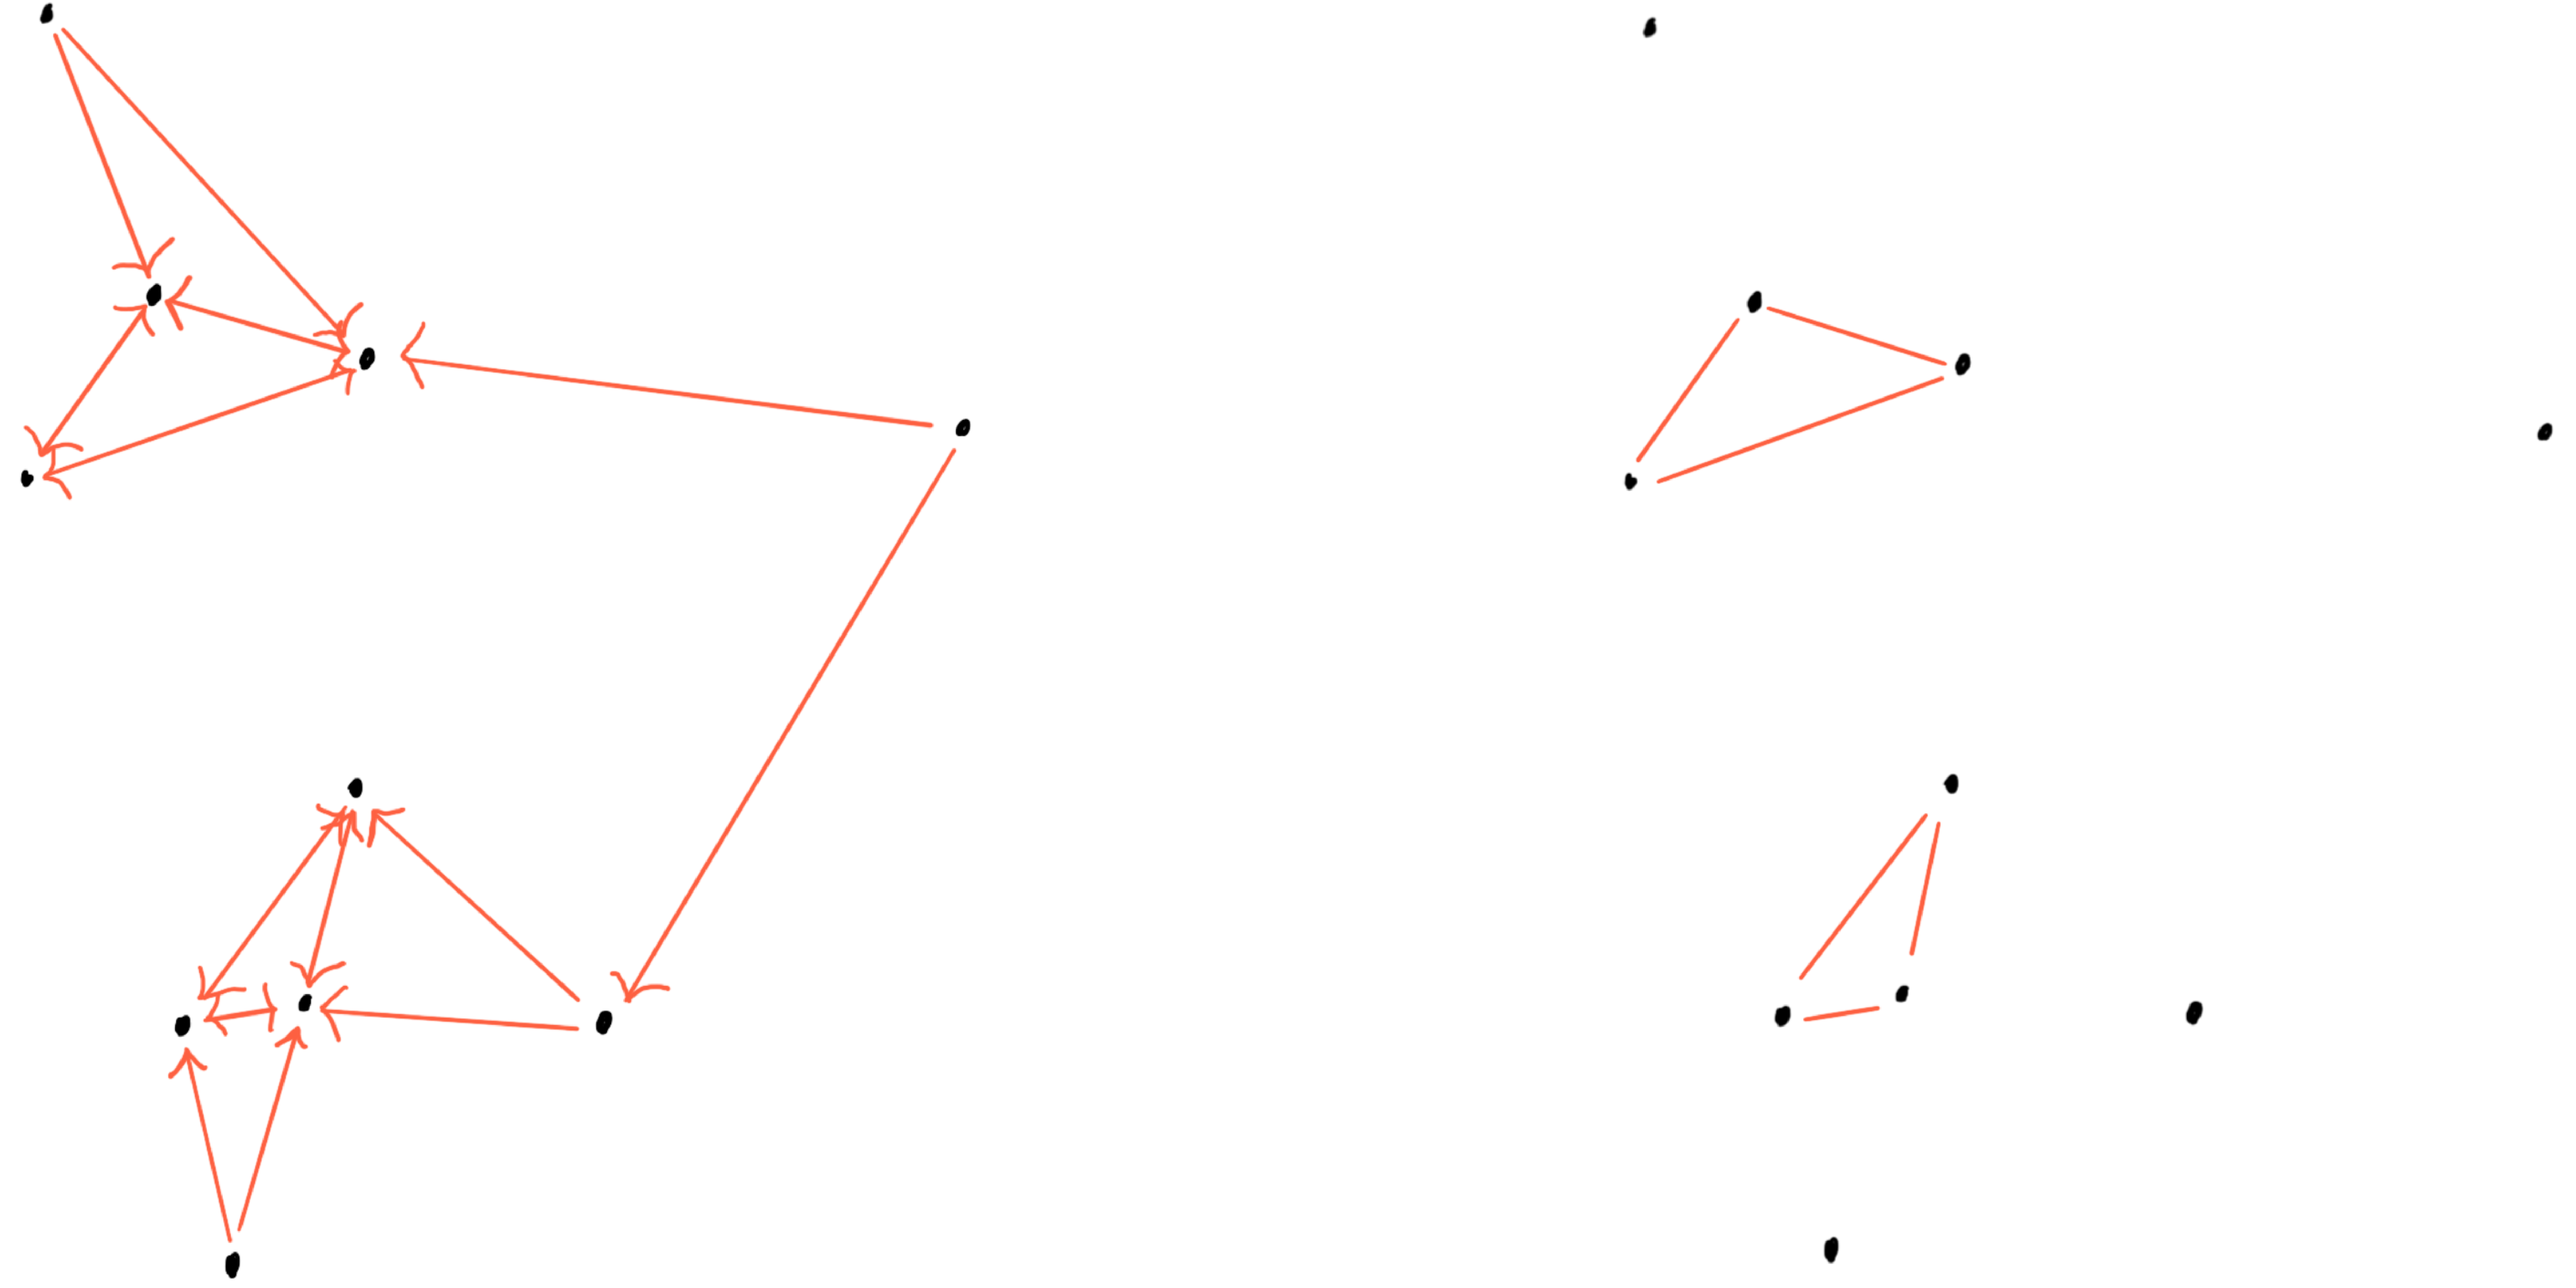
\includegraphics[width = 15cm]{mknn}
	\caption{The 2NN and M2NN graphs for the same dataset. Note how the M2NN graph is
	undirected and has a lot less edges.}
	\label{fig:mknn}
\end{figure}

Looking at \cref{fig:mknn} we see the 2-nearest neighbours and mutual 2-nearest neighbours
graphs for the same point cloud. In a \( k \)NN	 graph, it is always the case that every
vertex has \( k \) edges, which means that even points which are far away from any cluster
are connected to some other points. This is not very useful if we wish to detect outliers.
However, when taking the \emph{mutual} version, many of this edges disappear. Indeed, now,
for an outlier to become connected to a cluster a higher \( k \) will be required so that
every point within the cluster has become connected to all of its immediate neighbours and
is forced to ``look'' outside the cluster for additional neighbours. This idea of waiting
for a higher \( k \) is exactly the one we exploit when combining the \MKNN graph with
persistent homology, for outliers will presumably become classes in	\( H_0 \) with few
elements and with a long lifetime. 

\section{The steps of the algorithm}
The whole process from the input of the data until the output of the persistence barcode
is divided in three rough steps. First, the data is formatted into the expected format and
wrapped in a class which knows how to compute its \MKNN	graph for any \( k \). Then, the
filtration is built and suitably stored. Finally the actual computation of the persistence
homology takes place. We now describe each of these in detail and how the mathematical
considerations of each step are reflected in the implementation. The code for the whole
library is available at \url{https://github.com/arnaumas/mknn_homology/}. 

\subsection{Constructing the M\texorpdfstring{\( k \)}{k}NN graph}
The input is assumed to be in the form of a \textsf{NumPy} array of shape \( (N,d) \)
where \( N \) is the number of points and \( d \) the number of features or equivalently
the ambient dimension. This array is wrapped in an instance of the class \texttt{Cloud}
which implements a method to compute the \MKNN graph for a given \( k \). 

The procedure to encode this graph is as follows. First, the distance matrix, \( D \), for
the data set is computed. If we index the points of the cloud by \( C = \set{p_i}_{i =
1}^n \), then this matrix contains the difference between every pair of points:
\begin{equation*}
	D_{ij} = d(p_i, p_j). 
\end{equation*}
This can be done with \textsf{NumPy} and is implemented as a method of the \texttt{Cloud}
class. Then, again using \textsf{NumPy}, the indices of each
column of \( D \) are sorted into a new matrix such that the \( i \)-th column of this new
matrix lists the points of \( C \) by increasing order of distance to \( p_i \). In
particular, the first \( k \) are \( p_i \)'s \( k \)-th nearest neighbours. From this we
can then construct the adjacency matrix of the \( k \)NN graph, \( A \), which is in
general not symmetric since the graph is directed. The adjacency matrix of the \MKNN
graph, \( M \), is given by
\begin{equation*}
	M = A \odot A^\top
\end{equation*}
where \( \odot \) denotes the entrywise prodct. Indeed, we have
\begin{equation*}
	M_{ij} = A_{ij}A^\top_{ji} = A_{ij}A_{ji}
\end{equation*}
so that \( M_{ij} \) is nonzero if and only if both \( A_{ij} \) and \( A_{ji} \) are
nonzero, i.e. if there is an edge going from \( p_i \) to \( p_j \) and one from \( p_j	\) to \( p_i \). Furthermore 
\begin{equation*}
	M_{ij} = A_{ij}A_{ji} = A_{ji}A_{ij} = M_{ji}
\end{equation*}
which means that \( M \) is symmetric and therefore the adjacency matrix of an undirected
graph, as we claimed. This adjacency matrix is used to represent the \MKNN graph as a
\textsf{NetworkX} graph. \textsf{NetworkX} is a Python library which implements many
algorithms from graph theory. 

\subsection{Building the filtration}
The filtration used is based on the clique complex, see \cref{sec:clique complex}. For
every \( k \) we have the clique complex of the corresponding \MKNN graph. And letting
\( k \) from 0 to an appropriate upper bound we get a filtration. That this is indeed a
filtration is because the M\( (k-1) \)NN graph is a subgraph of the \MKNN graph. Indeed,
\( k-1 \) mutual nearest neighbours are in particular \( k \) mutual nearest neighbours.
This means cliques of the first are cliques of the latter, thus simplices of the clique
complex of the first are simplices of the clique complex of the latter, which proves the
claim. 

There are a couple caveats. First, we restrict the top dimension of the complex to the
ambient dimension \( d \), which means we will ignore any clique with more than \( d+1 \)
vetices. This is because homology at a dimension higher than this does not have much
geometric meaning (the points that would generate such simplicies are necessarily not
geometrically independent). Secondly, the matter of the upper bound for \( k \). A
generous upper boud is \( N-1 \) which results in the \MKNN graph being fully connected,
and the homology of the resulting complex is trivial (zero in all dimensions save for \(
H_0 \) which is of dimension 1). The problem is that the process of building the complex
does not scale well with \( k \) in terms of time, so it seems desirable to seek a lower
stopping point since most of the ``interesting'' fenomena will have, heuristically, already
happened somewhere between \( k = \lfloor N/2 \rfloor \) and \( k = N \). 

The work of constructing the filtration is packaged up in the \texttt{Filtration} class.
This class is passed an instance of \texttt{Cloud}. The most straightforward way to
represent a filtration is to simply store an ordered list of the \emph{new} simplices, in
this case cliques, which appear at every step. There are more efficient data structures
that can be used, see \cite{efficient, tidyset}, but since the data sets analysed are of small size, this more naive approach sufficed. 

The \textsf{NetworkX} package has methods which can compute every clique in a graph. In a
loop over \( k \) from \( 1 \) to the appropriate upper bound, the correspoinding \MKNN
graph is computed and a list of its cliques (of dimension less than or equal to \( d \))
is extracted. Of these, all those which are new are appended to a list. The
\texttt{Simplex} class wraps a clique as a list of its points as well as keeping track of the
step, \( k \), at which the clique is born. In addition it implements methods used in the
actual computation of the homology groups.

This list is then sorted by birth, such that cliques born earlier appear first, and
cliques with the same birth are sorted by increasing dimension. This guarantees that any
simplex is always preceded by its faces, which is required for later computations. 

\subsection{Justification of the algorithm}
The main idea of the algorithm used to compute the persistent homology is taken from
\cite{campos}. We now provide some justification as to why it works. 

Recall that the homology groups are defined as a quotient of the subgroup
of cycles by the subgroup of boundaries. But we can just as well consider the quotient of
the \emph{whole} chain group. More specifically, consider a filtration \( \set{K^i}_{i =
0}^N \) and its chain complex, \( C_\ast(K^i) \). We then have the corresponding boundary
morphisms,
\begin{equation*}
	\partial_p^i \colon C_p(K^i) \to C_{p-1}(K^i)
\end{equation*}
where the superscript \( i \) refers to the step of the filtration. The group of \( p
\)-cycles is \( \ker{\partial_p^i} \) and the group of \( p \)-boundaries is \(
\im{\partial_{p+1}^i} \). Since \( \partial_p \circ \partial_{p+1} = 0 \) the boundaries
are a subgroup of the cycles, which means the homology groups are well defined. But the
boundaries are a subgroup of \( C_p(K^i) \), which means we can
define what we will call \emph{prehomology groups} by
\begin{equation*}
	P_p(K^i) = C_p(K^i) / \im{\partial_{p+1}^i}
\end{equation*}
which is the result of identifying all homologous chains, not just the cycles. Let's write
\( \pi_p^i \) for the projection from \( C_p(K^i) \) onto \( P_p(K^i) \).

Now, because \( \im{\partial_{p+1}^i} \subseteq \ker{\partial_p^i} \), the boundary maps
factor through the prehomology groups, which means the following is well-defined
\begin{align*}
	\hombound{p}{i} \colon P_p(K^i) & \longto P_{p-1}(K^i) \\
	[c] & \longmapsto [\partial_p^i c]. 
\end{align*}
In particular,
\begin{equation*}
	\ker{\hombound{p}{i}} = H_p(K^i). 
\end{equation*}
Furthermore, essentially by definition, we have the identity
\begin{equation*}
	(\hombound{p}{i} \circ \pi_p^i)(\sigma) = (\pi_{p-1}^i \circ \partial_{p}^i)(\sigma)
\end{equation*}
and we will write \( b_p^i \) for this composition. 

Now, consider a \( p \)-simplex \( \sigma \) which is in \( K^i \) but not in any of the previous
steps of the filtration. Then two things can happen: either \( b^i(\sigma) \) is zero or
it is not. If it is zero then 


\subsection{Computing the homology}
The classes \texttt{Simplex} and \texttt{Chain} can be used to calculate with the chain
groups. As mentioned before, a \texttt{Simplex} simply wraps a clique as well as its
birth. It also has the property \texttt{faces}, which returns a list of the faces of the
simplex.

The elements of the chain group are linear combinations of simplices (of the same
dimension), but since we are working over \( \F_2 \), this amounts to a list of simplices,
which is what \texttt{Chain} stores\footnote{Infact we choose to work over \( \F_2 \)
precisely because of this reason.}. Furthermore, this class implements the addition of
chains which, again because the field we ar working over has characteristic 2, reduces to
taking the symmetric difference of the lists of simplices of the two chains we are adding.
Indeed, if we have two chains of the form \( c_1 = \sum_{i = 1}^{n} \epsilon_i \sigma_i \)
and \( c_2 = \sum_{i = 1}^{n} \delta_i \sigma_i \) with \( \epsilon_i, \delta_i \in \F_2
\), then
\begin{equation*}
	c_1 + c_2 = \sum_{i = 1}^{n} (\epsilon_i + \delta_i) \sigma_i
\end{equation*}
which means the coefficient of \( \sigma_i \) in \( c_1 + c_2 \) is \( \epsilon_j +
\delta_j \). And this will be 1 provided only one of \( \epsilon_j \) or \( \delta_j \) is
equal to 1, and will be 0 whenever \emph{both} \( \epsilon_j \) and \( \delta_j \) are 1
or 0. So \( \sigma_j \) will be present in \( c_1 + c_2 \) whenever it is present in \(
c_1 \) or \( c_2 \), but not both. 

This makes it very easy to implement the boundary morphisms. For a single simplex, wrap
the list of faces inside a \texttt{Chain} object. And for a larger chain, add up the
boundaries of each of its constituent simplices. Again, this works because we are taking
coefficients from \( \F_2 \), so that, as explained in \cref{sec:different coefficients}
the alternating signs that appear in the definition of the boundary all disappear. 




\end{document}
